\section{EiffelStudio}
\label{implementation_eiffelstudio}
The textual \textsc{bon} tool is implemented in a view (the reason for this will be explained in section \ref{why_a_view}). Switching between views is taken care of by a \textsc{eb$\textunderscore$development$\textunderscore$window}, through telling a \textsc{eb$\textunderscore$class$\textunderscore$text$\textunderscore$formatter} that it is now active. Such a \textsc{eb$\textunderscore$class$\textunderscore$text$\textunderscore$formatter} represents a view, but the \textsc{eb$\textunderscore$development$\textunderscore$window} does not know which \textsc{eb$\textunderscore$class$\textunderscore$text} \textsc{$\textunderscore$formatter} it is switching to as this is done polymorphic. It simply iterates through all its available formatters and waits for a \textit{selected}-flag to be set. When adding a new view one therefore has to add the new view to this collection of formatters and make sure the \textsc{ui} sets its \textit{selected}-flag appropriately. When the right \textsc{eb$\textunderscore$class$\textunderscore$text$\textunderscore$formatter} has been found the \textsc{format} feature will be invoked in order to start the formatting process for the chosen view.

\paragraph{}
This is how the \textsc{bon} tool is hooked into EiffelStudio as a view. The \textsc{bon} formatters, \textsc{textual$\textunderscore$ bon$\textunderscore$formal$\textunderscore$formatter} and \textsc{textual$\textunderscore$bon$\textunderscore$infor- mal$\textunderscore$formatter}, are added to the \textsc{eb$\textunderscore$development$\textunderscore$window}. A \textsc{eb$\textunderscore$sha- red$\textunderscore$format$\textunderscore$tables} then binds the formatter and a \textsc{class$\textunderscore$text$\textunderscore$formatter} together by instantiating the \textsc{class$\textunderscore$text$\textunderscore$formatter}, setting certain meta data on it and telling it to format with the formatter. This \textsc{class$\textunderscore$text$\textunderscore$formatter} executes the formatter, which hands over an abstract eiffel syntax representation of the class in scope to a \textsc{textual$\textunderscore$bon$\textunderscore$formal$\textunderscore$output$\textunderscore$strategy} which starts the actual extraction of \textsc{bon}. An overview of  an example of this structure for formal textual \textsc{bon} can be seen in figure \ref{fig:extractor_structure}.
\begin{figure}[h]
\centerline{
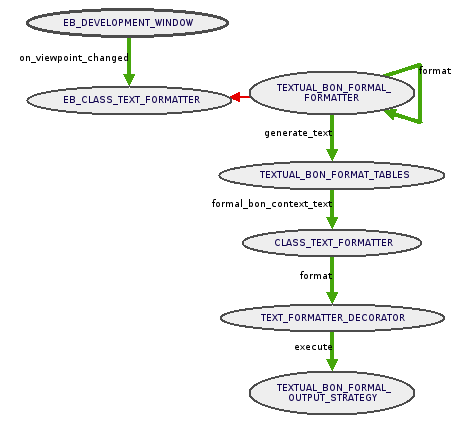
\includegraphics[scale=0.7]{images/BON-extractor-structure-large.png}
}
\caption{Structure of the BON extractor's interaction with EiffelStudio for formal BON.}
\label{fig:extractor_structure}
\end{figure}